\documentclass[12pt]{article}
\usepackage[italian]{babel}
\usepackage[utf8]{inputenc}
\usepackage{hyperref}
\usepackage{graphicx}
\usepackage{float}
\usepackage{listings}
\usepackage{indentfirst}
\usepackage{caption}
\usepackage{subcaption}
\usepackage{amsmath}
\usepackage{enumerate}
\usepackage{multicol}

\title{QSVM for Sentiment Analysis}
\author{Mario Bifulco (881727)}
\date{UniTo, 2023/2024}

\begin{document}

\maketitle

\section{Disclamer}

The following file is not intended to be read by third parties, 
its purpose is to keep track of the work done during the thesis. 
For this reason, I will not edit the style of the writing and will present what I have done in Italian.

\section{Research questions}

Quali sono le finalità di questa tesi? A quali domande vorrei rispondere?

\paragraph{Le QPU sono valide per task di machine learning?} 
La promessa del quantum computing è quella di velocizzare problemi “difficili" su calcolatori classici.
Ad oggi il quantum adiabatic computing permette di risolvere problemi di ottimizzazione di natura quadratica.
I problemi di machine learning si possono quasi sempre ridurre all'ottimizzazione, 
è quindi possibile trarre \emph{vantaggi} dagli approcci quantistici?

La domanda in questo momento è ambigua, innanzitutto bisogna decidere su quale aspetto effettuare il confronto:
\begin{enumerate}
    \item Tempo di apprendimento,
    \item Qualità della soluzione,
    \item Semplicità nella riscrittura del problema.
\end{enumerate}
Bisogna inoltre considerare che le attuali QPU sono estremamente limitate, 
quindi bisogna considerare anche \emph{problemi di scalabilità}.

Questo probetto di tesi prende in esame le macchine a vettori di supporto (SVM) in cui, per definizione, 
esiste un problema di ottimizzazione quadratico nell'apprendimento.

La scelta di questa architettura rispetto ad altre non è dovuta solo al naturale collegamento con i problemi ideali per le QPU,
le SVM si sono rivelate architetture molto versatili, inoltre è possibile dimostrare matematicamente che il meccanismo di attenzione dei Transformer è equivalente al processo di ottimizzazione del margine delle SVM.
Ottenere quindi buoni risultati potrebbe portare ad una prima implementazione dell'architettura Transformer su macchine quantistiche.

\section{Dataset}

La tesi si articola in una riscrittura su architettura quantistica delle SVM per il task di sentiment analysis (SentA).

Come dataset per il problema si è scelto \textsc{TweetEval}, nel sottoinsieme \textsc{Sentiment}.
Questo dataset contiene frasi di Twitter suddivise in tre split, train, validation e test, 
ogni esempio è etichettato con una delle tre classi (positivo, negativo, neutro).

Siccome le SVM sono classificatori binari gli esempi di classe neutra sono stati scartati, 
e tra i rimanenti è stata applicata una normalizzazione per avere una distribuzione delle classi uniforme.
Nota: le classi di \textsc{TweetEval} sono positiva (2) e negativa (0), 
per riportare agli standard utilizzati dalle SVM sono state trasformate in 1 (positiva) e -1 (negativa).

Una volta limato il dataset per gli scopi del progetto è stato necessario trasformare le frase in embedding,
questo perché le architetture di machine learning non sono in grado di elaborare direttamente il testo, ma occorre una rappresentazione numerica.

Una prima trasformazione è stata effettuata tramite l'utilizzo di SentenceBert, 
una architettura Transformer che permette di ottenere l'embedding di una frase.

Successivamente è possibile sperimentare con eltre forme di embedding quali ad esempio:
\begin{itemize}
    \item Un senso mediano estratto da Word2Vec. Word2Vec permette di associare un embedding per ogni parola, ed è stato dimostrato come sia possibile svolgere “aritmetica di base" sugli embedding.
    \item Embedding custom estratti a partire dalle caratteristiche della frase decise dallo sviluppatore.
\end{itemize}

\paragraph{Dataset di test}
Per poter testare e visualizzare durante la fase di sviluppo sono stati creati due dataset di supporto.

\begin{figure}[H]
    \centering
    \begin{subfigure}{.49\textwidth}
      \centering
      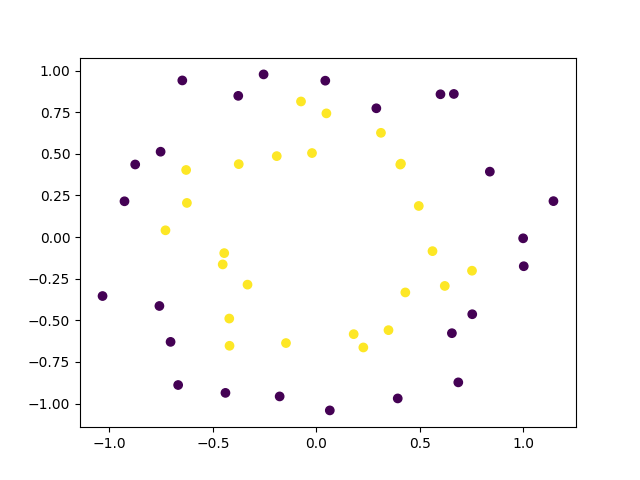
\includegraphics[width=\linewidth]{img/dummy.png}
      \caption{\textsc{Dummy} dataset}
    \end{subfigure}
    \begin{subfigure}{.49\textwidth}
      \centering
      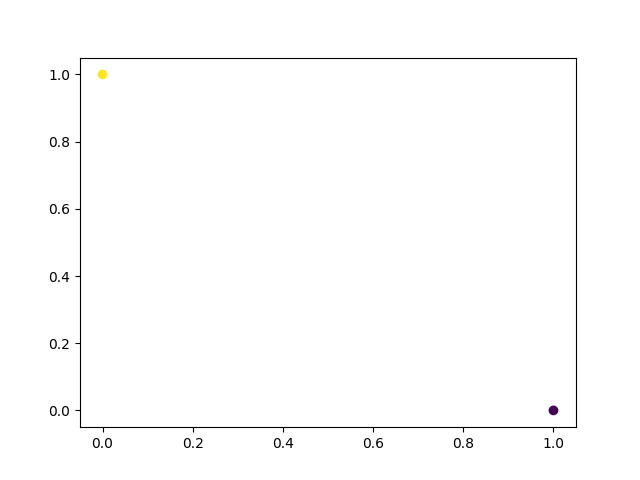
\includegraphics[width=\linewidth]{img/toy.png}
      \caption{\textsc{Toy} dataset}
    \end{subfigure}
\end{figure}

\section{Implementazione dell'architettura}

Per svolgere una prima fase eplorativa l'architettura delle SVM è stata testata con il dataset \textsc{Dummy} in tre casi:
\begin{itemize}
  \item Usando le librerie allo stato dell'arte (SK-Learn),
  \item Implementando il problema di ottimizzazione e risolvendolo con un ottimizzatore classico (Gurobi),
  \item Implementando il problema per una soluzione su QPU tramite i solver ibridi di DWave.
\end{itemize}

\paragraph{SK-Learn} La classe SVC implementa il modello di suppor vector machine per la classificazione.
Questo metodo risulta essere il più veloce come tempo di esecuzione per via dei binding a librerie scritte nativamente in \textsc{C++}.
Bisogna notare come il modello di SVM implementato sia leggermente diverso rispetto alla formulazione standard, 
questa differenza è dovuta al fatto che nelle SVC viene applicata una regolarizzazione di tipo L2,
con la finalità di stabilizzare la distribuzione dei risultati.

\begin{figure}[H]
  \centering
  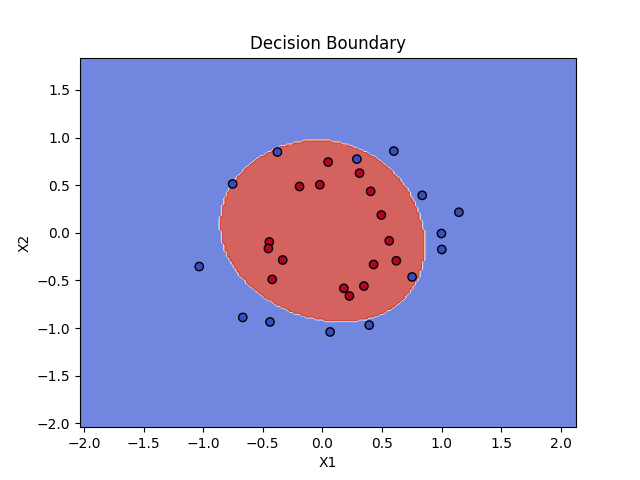
\includegraphics[width=\linewidth]{img/decision_boundary_sklearn.png}
\end{figure}

\paragraph{Gurobi} Per la scrittura del problema di ottimizzazione è stata utilizzata la libreria \textsc{PyOmo},
che permette di scrivere i problemi di soddisfacimento di vincoli in modo intuitivo e facilmente comprensibile in quando “vicino" a come gli stessi problemi verrebbero scritti in forma matematica.
Una volta scritto il problema è possibile inizializzare un solver general purpose (in questo caso Gurobi) e richiedere la soluzione.
È importante sottolineare che, per quanto ottima a livello di leggibilità e utilizzo, 
\textsc{PyOmo} aggiunge overhead durante la risoluzione in quanto il problema viene prima rappresentato con un formato interno e poi convertito per essere passato al solver selezionato.

\begin{figure}[H]
  \centering
  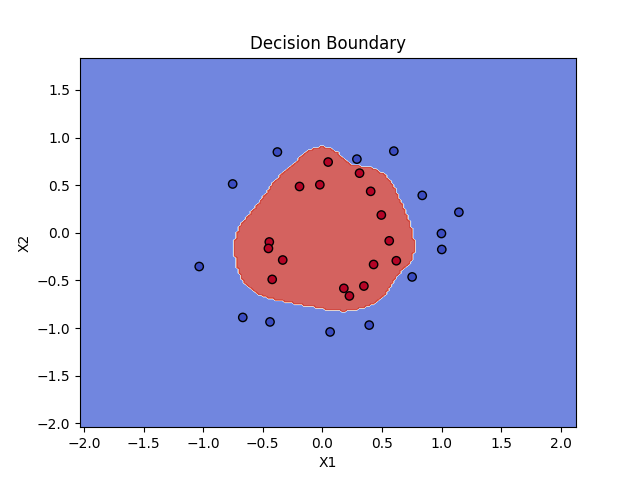
\includegraphics[width=\linewidth]{img/decision_boundary_gurobi.png}
\end{figure}

I risultati prodotti sono paragonabili a quanto ottenuto tramite la libreria, e nonostante l'overhead di \textsc{PyOmo} il tempo di esecuzione rimane ragionevolmente contenuto.

\paragraph{D-Wave} Utilizzando il solver ibrido per i problemi di soddisfacimento di vincoli quadratici è possibile scrivere il problema di ottimizzazione in modo analogo a come avviene su \textsc{PyOmo} anche con le librerie D-Wave.
In questo caso il problema viene formalizzato, inviato al solver in remoto e viene restituita la risposta, con i livelli di energia associati.
Da notare che, per via dei limiti della libreria le variabili $\alpha$ non sono considerate a valori reali ma interi,
inoltre siccome i processi di ottimizzazione quantistica si aspettano problemi di minimizzazione, la funzione obiettivo è passata con segni invertiti rispetto al problema originale.

\begin{figure}[H]
  \centering
  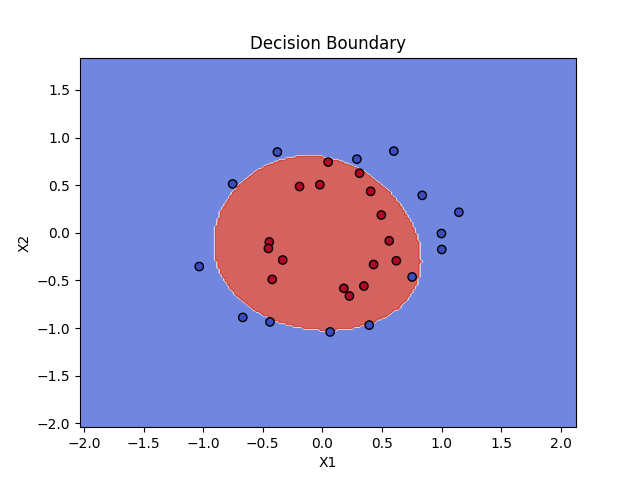
\includegraphics[width=\linewidth]{img/decision_boundary_dwave.png}
\end{figure}

È interessante notare che la discretizzazione delle variabili di ottimizzazione non incida sulla qualità del risultato, 
in quanto le metriche restituiscono sempre valori paragonabili.
In questo caso, seppure i valori numerici siano paragonabili, i tempi richiesti per la computazione aumentano sensibilmente, soprattutto per via della comunicazione con il solver remoto.

Ottenendo come risposta dal risolutore di D-Wave una lista di possibili soluzioni,
è possibile implementare una procedura concettualmente simile all'ensemble learning. 
Tuttavia tale implementazione non ha riscontrato vantaggi nella predizione di nuovi esempi, 
con l'unico risultato di aumentare in modo sensibile i tempi di calcolo necessari per inizializzare i diversi modelli.

\subsection{Problema di ottimizzazione per le SVM}

\paragraph{Problema primale}

\begin{align*}
  \text{minimize}_{w, t}\ & \frac{1}{2}||w||^2 \\
  \text{subject to } & y_i(w \cdot x_i - 1)\geq 1 \quad \forall i:1\leq i\leq n
\end{align*}

\paragraph{Problema duale con soft margin}

\begin{align*}
  \text{maximize}_\alpha\ & -\frac{1}{2}\sum_{i=1}^n\sum_{j=1}^n\alpha_i\alpha_jy_iy_jx_ix_j + \sum_{i=1}^n
\alpha_i \\
  \text{subject to } & 0 \leq \alpha_i \leq C \quad \forall i: 1\leq i\leq n \\
  & \sum_iy_i\alpha_i=0
\end{align*}

\paragraph{Kernel trick}

\begin{align*}
  \text{maximize}_\alpha\ & -\frac{1}{2}\sum_{i=1}^n\sum_{j=1}^n\alpha_i\alpha_jy_iy_jK(x_i, x_j) + \sum_{i=1}^n
\alpha_i \\
  \text{subject to } & 0 \leq \alpha_i \leq C \quad \forall i: 1\leq i\leq n \\
  & \sum_iy_i\alpha_i=0
\end{align*}

\paragraph{Dalla soluzione duale alla procedura di inferenza}

\subparagraph{Calcolo del bias}

$$b = \frac{\sum_{i=1}^n y_i - \sum_{j=1}^n(\alpha_jy_jK(x_i,x_j))}{n}$$

\subparagraph{Predizione}

$$f(x)=\sum_{i=1}^n\alpha_iy_iK(x_i, x) + b$$

\section{Analisi del \emph{minor embedding}}

Per la prima parte del lavoro di tesi l'analisi si è basata sull'uso del solver ibrido per problemi quadratici fornito da D-Wave.
Siccome la famiglia dei solver ibridi è \emph{closed-source} non è possibile indagare a fondo sui motivi della differenza di performance rispetto alla classe di SK-Learn.

Per questo motivo una successiva fase di analisi si è concentrata nel convertire i problemi da quadratici a binari (tramite i metodi di supporto forniti dalle librerie D-Wave) e analizzare il comportamento della soluzione su una QPU pura.
Il vantaggio è che in questo caso è possibile analizzare:
\begin{enumerate}
  \item La trasformazione del problema da CSP a grafo di variabili binarie,
  \item La ricerca del minore nel grafo dei qubit nella QPU disponibile,
  \item La variazione di performance in questo contesto.
\end{enumerate}

\paragraph{Conversione da CQM a BQM}

Per una soluzione “migliore" e per ridurre il carico sulla QPU, la documentazione di D-Wave consiglia di effetturare una fase di Pre-Solving.
Questa procedura dovrebbe svolgere delle inferenze sulla struttura del problema e ridurre il quantitativo di qubit necessari per calcolare la nuova soluzione.
Tutta le trasformazioni applicate forniscono la garanzia di mantenere il problema ridotto equivalente all'originale.
Le strategia adottate per il Pre-Solving comprendono:
\begin{itemize}
  \item Rimozione di vincoli superflui,
  \item Rimozione di bias piccoli dalla funzione obiettivo e dai vincoli,
  \item Domain propagation.
\end{itemize}

Analizzando la trasformazione del problema si può notare come, per il modello di ottimizzazione delle SVM, la strategia di Pre-Solving conduca ad un grafo con più nodi rispetto a quello iniziale.
Questo può significare che le strategie proposte da D-Wave non siano particolarmente efficaci su problemi con una struttura simile a quella delle SVM.
Per questo motivo, le successive considerazioni considereranno una conversione da CQM a BQM senza applicare il Pre-Solving.

\paragraph{Minor Embedding}

Per la risoluzione di problemi tramite computazione quantistica adiabatica è necessario ricercare un grafo, nella rete di qubit, equivalente al problema di partenza.
La costruzione di tale embedding può essere svolta utilizzando nodi, archi e considerando diversi nodi come mapping di uno solo nel minore.

Il problema della ricerca del minore di un grafo quando sia il grafo di partenza che quello di arrivo sono parte dell'input è NP-completo.
Per questo motivo la strategia risolutiva di D-Wave sfrutta un'euristica che dichiarano funzionare ragionevolmente bene per grafi sparsi.

Il problema delle SVM è per sua natura un grafo completo, bisogna quindi valutare l'efficacia dell'euristica in questo contesto.
Dalla documentazione viene anche proposto una strategia di embedding a clique, al momento però sembra non funzionare a dovere, quindi i commenti saranno riferiti solo alla strategia standard proposta.

Usando il dataset \textsc{Dummy} si registrano tempi necessari per l'embedding incompatibili con la velocità di risoluzione del solver ibrido,
inoltre testando la creazione dell'embedding con diversi seed randomici viene nella maggior parte dei casi restituita una soluzione non valida.
Questo comportamento può essere dovuto alla necessità di utilizzare la quasi totalità dei qubit anche con soluzioni semplici quali quella attesa con il dataset \textsc{Dummy}.

Si è quindi reso necessario l'utilizzo del dataset \textsc{Toy} per formulare delle ipotesi su un problema triviale e per poi applicarle in casi più complessi.

Il grafo generato dal dataset \textsc{Toy} contiene 8 nodi, considerando solo due esempi e le variabili $\alpha$ discretizzate e con upper-bound a 10.
Si può facilmente dedurre come sia necessario un numero di nodi pari al numero di esempi (o equivalentemente il numero di $\alpha$) moltiplicato per il numero di bit necessario per rappresentare ogni variabile $\alpha$.
$$\#nodes = \#examples (\lfloor\log_2(UB_\alpha)\rfloor+1)$$
Ovviamente il numero di nodi nel grafo target può aumentare per via delle catene di qubit che si occupano di rappresentare un singolo nodo del grafo minore.

Eseguendo la procedura di Minor-Embedding, utilizzando come seed randomico i primi 1000 numeri primi, è seguita un'analisi sugli embedding prodotti,
cercando di identificare quanto frequentemente seed diversi producessero lo stesso embedding e la posizione sul grafo \emph{pegasus} di tali embedding.

Solo in 16 dei 1000 casi analizzati si riscontrano embedding identici sia nella forma che nella posizione, questo avviene per le coppie di seed:
\begin{multicols}{4}
  \begin{itemize}
    \item 19 - 6451
    \item 107 - 4871
    \item 419 - 6947
    \item 859 - 2789
    \item 967 - 7523
    \item 1237 - 6967
    \item 1699 - 6703
    \item 1709 - 4789
    \item 1979 - 5107
    \item 2389 - 3761
    \item 2917 - 3041
    \item 3571 - 3793
    \item 3877 - 6709
    \item 4027 - 6199
    \item 4813 - 7789
    \item 5179 - 6737
  \end{itemize}
\end{multicols}

Invece cercando embedding con le stesse forme, ammettendo quindi posizioni diverse nel grafo, si ottiene un numero considerevolmente maggiore di riscontri.

Vengono trovati un totale di 156 gruppi di grafi identici, la maggioranza dei quali con un numero di elementi $\leq 10$.
Il gruppo più frequente contiene 42 elementi, e il grafo prodotto assume la seguente forma:

\begin{figure}[H]
  \centering
  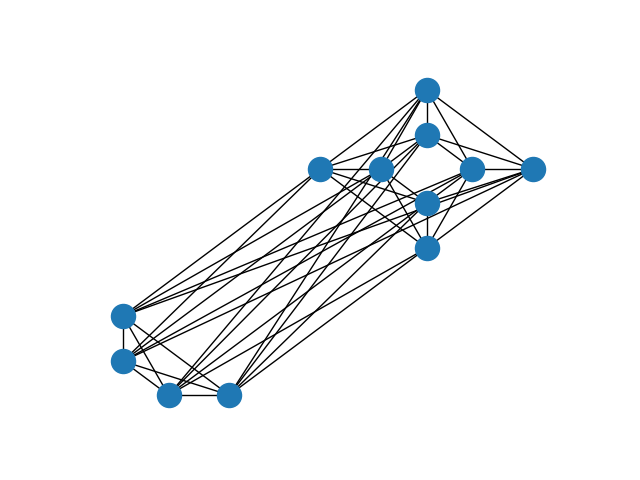
\includegraphics[width=\linewidth]{img/317.png}
\end{figure}

Si può notare come il numero di nodi sia maggiore di quanto conteggiato precedentemente, questo perché sono presenti 4 coppie di nodi che collassano in un unico nodo nel grafo minore.
Nella figura riportata non sono segnalati gli archi che collegano una catena di nodi in quanto questo può variare in base al seed randomico fornito.

Per analizzare la distribuzione sul grafo pegasus sono stati delineati 16 ripartizioni uguali, 
verificando su quali fosse più probabile trovare l'embedding.

Si osserva la seguente distribuzione:

\begin{figure}[H]
  \centering
  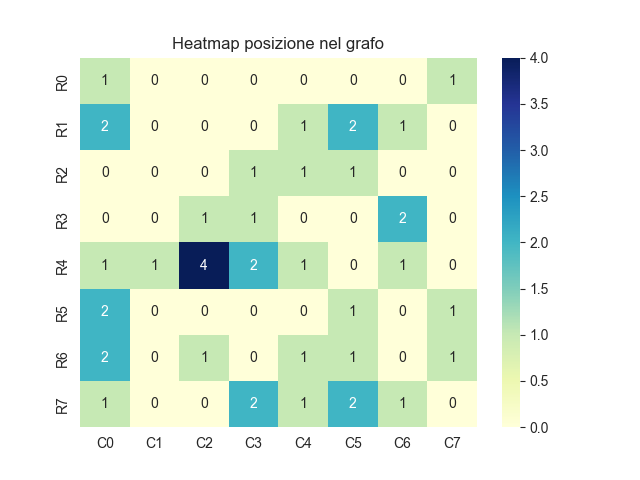
\includegraphics[width=\linewidth]{img/heatmap.png}
\end{figure}

Come si può notare, non si evincono differenze sostanziali.

\paragraph{Scalabilità del problema}
Oltra ad una analisi di alto livello sugli embedding prodotti dal dataset \textsc{Toy} è interessante verificare fino a che punto è possibile fare crescere il problema di ottimizzazione prima di superare i limiti fisici della QPU.

Per questo tipo di sperimentazione si definisce una dataset composto da $n$ punti, i punti sono disposti su una linea e gli $n/2$ punti della classe positiva sono specchiati per generare i punti della classe negativa.

Con una dataset facilmente definibile in modo programmatico è possibile testare le diverse combinazioni di: 
\begin{itemize}
  \item Seed randomico,
  \item Dimensione del dataset,
  \item Upper bound al valore delle variabili di ottimizzazione,
  \item Applicazione della strategia di Pre-Solving 
\end{itemize}

Dei diversi risultati raccolti si riportano i seguenti grafi:
\begin{enumerate}
  \item Crescita nel numero di nodi dell'embedding con 32 esempi e senza pre-solving
  \item Tempo richiesto per il calcolo dell'embedding
  \item Crescita nel numero di nodi dell'embedding fissando il limite di $\alpha$ a 3 e senza pre-solving
  \item Tempo richiesto per il calcolo dell'embedding
\end{enumerate}

\begin{figure}[H]
  \centering
  \subfloat[]{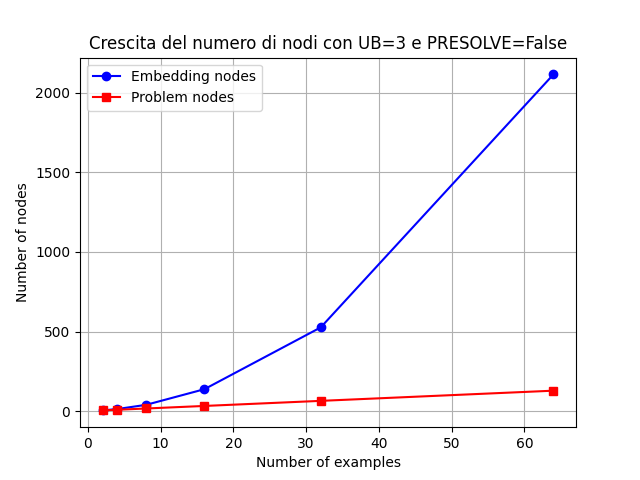
\includegraphics[width=.48\textwidth]{img/example_growth.png}}\quad
  \subfloat[]{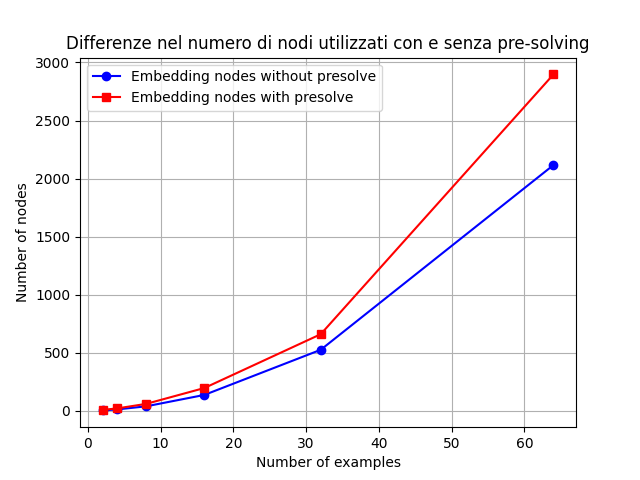
\includegraphics[width=.48\textwidth]{img/presolve.png}}\\
  \subfloat[]{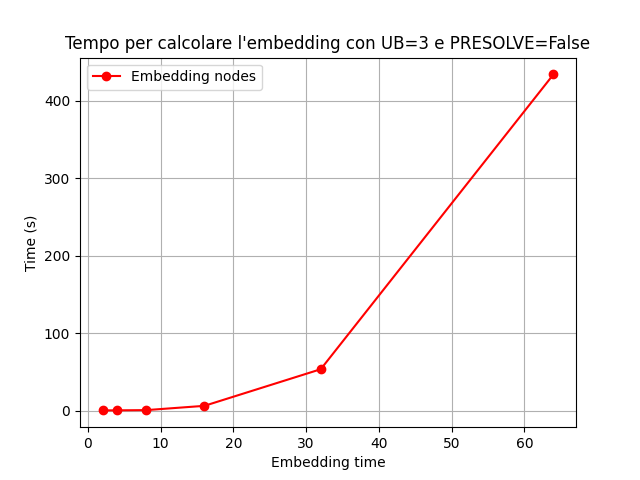
\includegraphics[width=.48\textwidth]{img/time.png}}\quad
  \subfloat[]{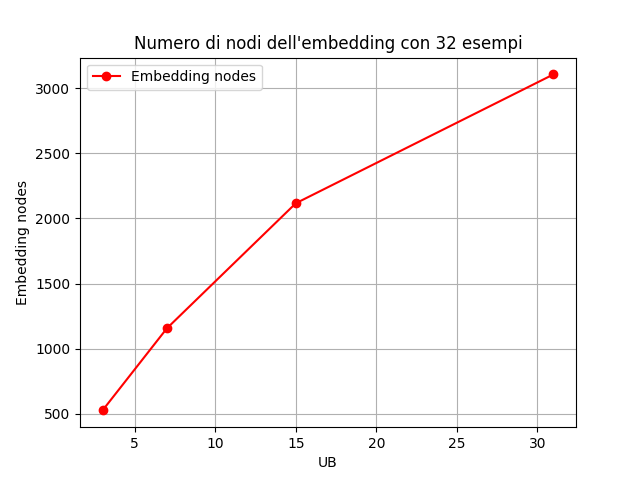
\includegraphics[width=.48\textwidth]{img/ub_growth.png}}
\end{figure}

Considerando che i nodi disponibili nella QPU di D-Wave sono 5627 (grafo pegasus) si possono trarre alcune considerazioni:
\begin{itemize}
  \item L'utilizzo diretto della QPU non scala per un numero di esempi significativo,
  \item La procedura di minor-embedding, per quanto guidata da un'euristica, non porta a buoni risultati nel problema affrontato,
  \item La componente classica nel solver ibrido ha un ruolo cruciale per permettere al problema di scalare su dataset reali.
\end{itemize}

\paragraph{Analisi delle performance}

\end{document}